\chapter{}

\section{Парабола (продолжение)}

\begin{theorem}[Касательная к параболе]
	$$ y^2 = 2px $$
    $ (x_0, y_0) $ -- точка на параболе \\
    $ yy_0 = p(x + x_0) $ -- касательная
\end{theorem}

\begin{proof}
    $$ \begin{cases} yy_0 = p(x + x_0) \\ y^2 = 2px \end{cases} $$
    $$ px = yy_0 - px_0 $$
    $$ y^2 = 2yy_0 - 2px_0 = 2yy_0 - y_0^2 $$
    $$ y^2 - 2yy_0 + y_0^2 = 0 $$
    $$ (y - y_0)^2 = 0 $$
\end{proof}

\begin{theorem}[Оптическое свойство параболы]
    \hfill \\
	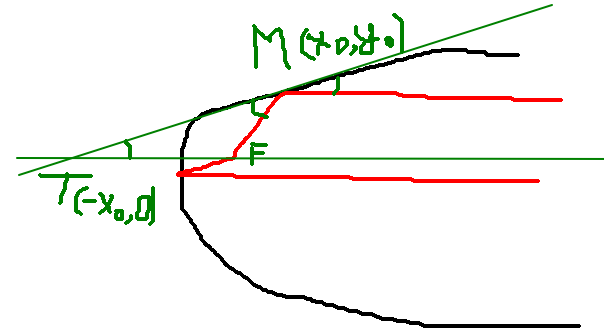
\includegraphics[scale=0.5]{1}
\end{theorem}

\begin{proof}
	$$ TF \stackrel?= FM $$
    $$ TF = x_0 + \frac{p}2 $$
    $$ FM = |M, \text{директриса} | = x_0 + \frac{p}2 $$
\end{proof}
\section{Классификация КВП (кривых второго порядка)}

Уравнение второго порядка: $ \underbrace{a_{11} x^2 + 2 a_{12} xy + a_{22} y^2}_{\text{квадратичная форма} (\ne 0)} + 2b_1 x + 2b_2 y + b_3 = 0 $ \\
Немного его упростим:
\begin{enumerate}
    \item Поворотом плоскости избавляемся от $ 2 a_{12} xy $:
    $$ a_{11} (x' \cos \alpha - y' \sin \alpha)^2 + 2 a_{12} (x' \cos \alpha - y' \sin \alpha)^2 \cdot (x' \sin \alpha + y' \cos \alpha) + a_{22} (x' \sin \alpha + y' \cos \alpha)^2 + ... $$
    $$ x'y' - 2a_{11} \cos \alpha \sin \alpha + 2 a_{12} (\cos^2 \alpha - \sin^2 \alpha) + 2 a_{22} \sin \alpha \cos \alpha = 0 $$
    $$ (a_{22} - a_{11}) \sin 2 \alpha + a_{12} \cos \alpha = 0 \quad | : \sin \alpha $$
    $$ a_{22} - a_{11} + 2 a_2 \ctg 2 \alpha = 0 $$
    \fbox{$ \ctg 2 \alpha = \frac{a_{11} - a_{22}}{2 a_{12}} $}
    $$ a_{11}' x'^2 + a_{22}' y'^2 + 2a_{11}'x' + 2b_2'y' \underset{(b_3' = b_3)}{ + b_3' = } 0 $$
    \item \begin{itemize}
        \item Если $a_{11}' \ne 0 $, то считаем $b_1' = 0$:
        $$ a_{11}'x^2 + 2b_1'x = a_{11} (x^2 + 2 \frac{b_1'}{a_{11}'}x + \frac{b'^2}{a_{11}'^2}) $$
        \item Если $a_{11}' = 0$, то считаем $b_3' = 0$
          \end{itemize}

\end{enumerate}

\subsubsection{Полярная система координат. Поворот}
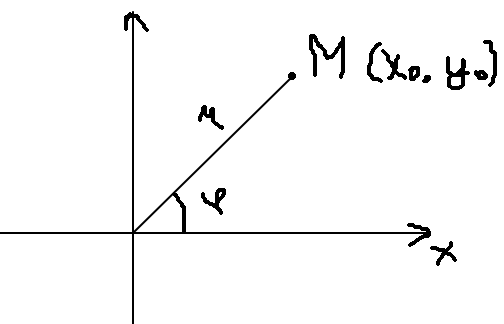
\includegraphics[scale=0.8]{2} \\
$ (r, \vphi) $ -- полярные координаты $ M $ \\
Переход:
$$ \begin{cases} x = r \cos \vphi \\ y = r \cos \vphi \end{cases} $$
Поворот на $\alpha$:
$$ x' = r \cos \vphi' = r \cos (\vphi - \alpha) = r \cos \vphi \cdot \cos \alpha + r \sin \vphi \cdot \sin \alpha = x \cos \alpha + y \sin \alpha $$
$$ y' = ... = - x \sin \alpha + y \cos \alpha $$
